\subsection{Experimental Setup}
\label{sec:setup}

\subsubsection{System used}

We employ a server equipped with two Intel Xeon Gold 6226R processors, each featuring $16$ cores running at a clock speed of $2.90$ GHz. Each core is equipped with a $1$ MB L1 cache, a $16$ MB L2 cache, and a $22$ MB shared L3 cache. The system is configured with $376$ GB RAM and set up with CentOS Stream 8.


\subsubsection{Configuration}

We use 32-bit integers for vertex ids and 32-bit float for edge weights but use 64-bit floats for computations and hashtable values. We utilize $64$ threads to match the number of cores available on the system (unless specified otherwise). For compilation, we use GCC 8.5 and OpenMP 4.5.


\subsubsection{Dataset}

The graphs used in our experiments are given in Table \ref{tab:dataset}. These are sourced from the SuiteSparse Matrix Collection \cite{suite19}. In the graphs, number of vertices vary from $3.07$ to $214$ million, and number of edges vary from $25.4$ million to $3.80$ billion. We ensure edges to be undirected and weighted with a default of $1$.

\begin{table}[hbtp]
  \centering
  \caption{List of $13$ graphs obtained SuiteSparse Matrix Collection \cite{suite19} (directed graphs are marked with $*$). Here, $|V|$ is the number of vertices, $|E|$ is the number of edges (after adding reverse edges), $D_{avg}$ is the average degree, and $|\Gamma|$ is the number of communities obtained with \textit{GVE-Leiden}.\ignore{In the table, B refers to a billion, M refers to a million and K refers a thousand.}}
  \label{tab:dataset}
  \begin{tabular}{|c||c|c|c|c|}
    \toprule
    \textbf{Graph} &
    \textbf{\textbf{$|V|$}} &
    \textbf{\textbf{$|E|$}} &
    \textbf{\textbf{$D_{avg}$}} &
    \textbf{\textbf{$|\Gamma|$}} \\
    % \textbf{$1 - \Gamma_G$} \\
    \midrule
    \multicolumn{5}{|c|}{\textbf{Web Graphs (LAW)}} \\ \hline
    indochina-2004$^*$ & 7.41M & 341M & 41.0 & 5.00K \\ \hline  % & \num{4.7e-4} & 2.9 GB
    uk-2002$^*$ & 18.5M & 567M & 16.1 & 43.1K \\ \hline  % & \num{9.6e-5} & 16 GB
    arabic-2005$^*$ & 22.7M & 1.21B & 28.2 & 3.80K \\ \hline  % & \num{5.5e-4} & 11 GB
    uk-2005$^*$ & 39.5M & 1.73B & 23.7 & 21.2K \\ \hline  % & \num{9.6e-5} & 16 GB
    webbase-2001$^*$ & 118M & 1.89B & 8.6 & 2.77M \\ \hline  % & \num{7.3e-7} & 18 GB
    it-2004$^*$ & 41.3M & 2.19B & 27.9 & 5.24K \\ \hline  % & \num{3.8e-4} & 19 GB
    sk-2005$^*$ & 50.6M & 3.80B & 38.5 & 3.75K \\ \hline  % & \num{5.8e-4} & 33 GB
    \multicolumn{5}{|c|}{\textbf{Social Networks (SNAP)}} \\ \hline
    com-LiveJournal & 4.00M & 69.4M & 17.4 & 2.33K \\ \hline  % & \num{7.9e-4} & 480 MB
    com-Orkut & 3.07M & 234M & 76.2 & 33 \\ \hline  % & \num{6.7e-2} & 1.7 GB
    \multicolumn{5}{|c|}{\textbf{Road Networks (DIMACS10)}} \\ \hline
    asia\_osm & 12.0M & 25.4M & 2.1 & 2.56K \\ \hline  % & \num{8.4e-4} & 200 MB
    europe\_osm & 50.9M & 108M & 2.1 & 3.61K \\ \hline  % & \num{6.6e-4} & 910 MB
    \multicolumn{5}{|c|}{\textbf{Protein k-mer Graphs (GenBank)}} \\ \hline
    kmer\_A2a & 171M & 361M & 2.1 & 19.4K \\ \hline  % & \num{9.4e-5} & 3.2 GB
    kmer\_V1r & 214M & 465M & 2.2 & 8.60K \\ \hline  % & \num{3.2e-4} & 4.2 GB
  \bottomrule
  \end{tabular}
\end{table}
% We convert directed graphs (marked with $*$) to undirected by duplicating edges in the reverse direction, and set the weight of each edge to $1$. and $F_{size}$ is size of the \textit{MatrixMarket} file

% \input{src/fig-leiden-compare}
% \input{src/fig-gve-compare}




\subsection{Comparing Performance of GVE-Leiden}

TODO.

% \input{src/fig-leiden-splits}
% \input{src/fig-leiden-hardness}
\begin{figure}[hbtp]
  \centering
  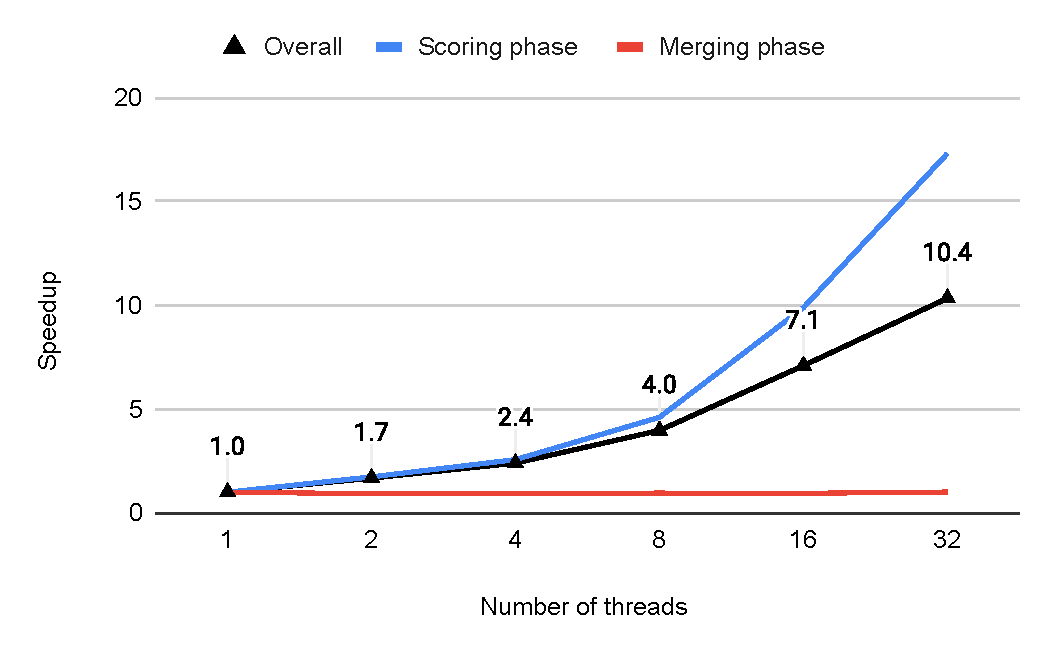
\includegraphics[width=0.98\linewidth]{out/strong-scaling-speedup.pdf} \\[-2ex]
  \caption{Overall speedup of our approach of \textit{Disregarding Large Hubs (DLH)} for link prediction, and its phases (obtaining edges with top-k scores per thread, and merging scores from each thread into a common scoreboard), with $10^{-2}|E|$ unobserved edges, with increasing number of threads (in multiples of 2). Increasing the number of threads causes work in the merging phase to increase,\ignore{thus} leading to a poor speedup.}
  \label{fig:strong-scaling}
\end{figure}





\subsection{Analyzing Performance of GVE-Leiden}

TODO.




\subsection{Strong Scaling of GVE-Leiden}

TODO.
